\documentclass[tikz]{standalone}  
\usepackage{physics}
\usepackage{amsmath}
\usepackage{tikz}
\usepackage{mathdots}
\usepackage{yhmath}
\usepackage{cancel}
\usepackage{color}
\usepackage{siunitx}
\usepackage{array}
\usepackage{multirow}
\usepackage{amssymb}
\usepackage{gensymb}
\usepackage{tabularx}
\usepackage{extarrows}
\usepackage{booktabs}
\usetikzlibrary{fadings}
\usetikzlibrary{patterns}
\usetikzlibrary{shadows.blur}
\usetikzlibrary{shapes}

\begin{document}
	
	
	\tikzset{every picture/.style={line width=0.75pt}} %set default line width to 0.75pt        
	
	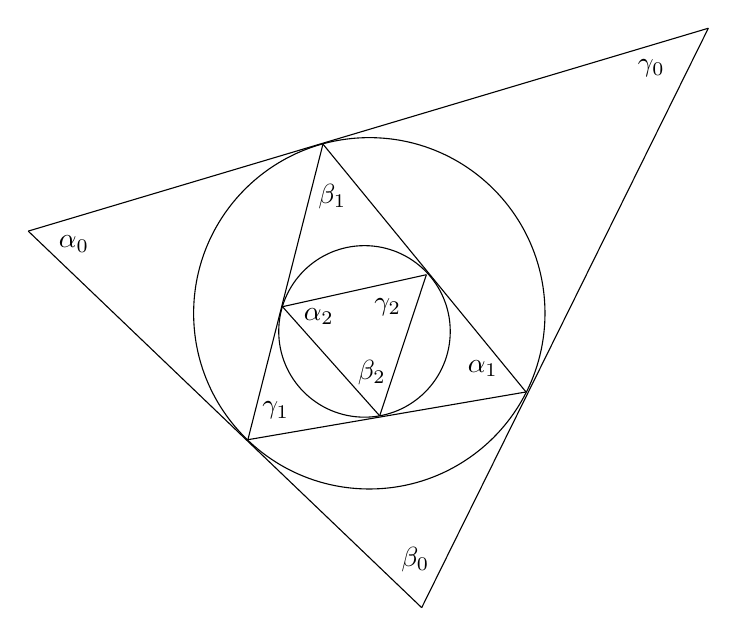
\begin{tikzpicture}[x=0.75pt,y=0.75pt,yscale=-1,xscale=1]
		%uncomment if require: \path (0,300); %set diagram left start at 0, and has height of 300
		
		%Shape: Ellipse [id:dp676279325262423] 
		\draw   (164.69,148.52) .. controls (164.69,101.77) and (202.58,63.88) .. (249.33,63.88) .. controls (296.07,63.88) and (333.97,101.77) .. (333.97,148.52) .. controls (333.97,195.26) and (296.07,233.16) .. (249.33,233.16) .. controls (202.58,233.16) and (164.69,195.26) .. (164.69,148.52) -- cycle ;
		%Straight Lines [id:da20400707194881285] 
		\draw    (85,108.92) -- (274.57,290.33) ;
		%Straight Lines [id:da233973159486768] 
		\draw    (85,108.92) -- (412.67,11.17) ;
		%Straight Lines [id:da5167067698316676] 
		\draw    (274.57,290.33) -- (412.67,11.17) ;
		%Straight Lines [id:da9188340275571596] 
		\draw    (227,67) -- (324.83,186.42) ;
		%Straight Lines [id:da0683160101616096] 
		\draw    (227,67) -- (190.83,209.42) ;
		%Straight Lines [id:da8075017485973699] 
		\draw    (190.83,209.42) -- (324.83,186.42) ;
		%Shape: Ellipse [id:dp4974759079830361] 
		\draw   (205.69,157.24) .. controls (205.69,134.42) and (224.19,115.92) .. (247.01,115.92) .. controls (269.83,115.92) and (288.33,134.42) .. (288.33,157.24) .. controls (288.33,180.06) and (269.83,198.56) .. (247.01,198.56) .. controls (224.19,198.56) and (205.69,180.06) .. (205.69,157.24) -- cycle ;
		%Straight Lines [id:da11678873766478703] 
		\draw    (207.5,145.33) -- (276.83,129.92) ;
		%Straight Lines [id:da5436533959662725] 
		\draw    (207.5,145.33) -- (254.33,197.92) ;
		%Straight Lines [id:da6438982692833218] 
		\draw    (276.83,129.92) -- (254.33,197.92) ;
		
		% Text Node
		\draw (98.5,110) node [anchor=north west][inner sep=0.75pt]    {$\alpha _{0}$};
		% Text Node
		\draw (295.5,170) node [anchor=north west][inner sep=0.75pt]    {$\alpha _{1}$};
		% Text Node
		\draw (216.5,145) node [anchor=north west][inner sep=0.75pt]    {$\alpha _{2}$};
		% Text Node
		\draw (377.5,25) node [anchor=north west][inner sep=0.75pt]    {$\gamma _{0}$};
		% Text Node
		\draw (196.5,190) node [anchor=north west][inner sep=0.75pt]    {$\gamma _{1}$};
		% Text Node
		\draw (250.5,140) node [anchor=north west][inner sep=0.75pt]    {$\gamma _{2}$};
		% Text Node
		\draw (263.5,260) node [anchor=north west][inner sep=0.75pt]    {$\beta _{0}$};
		% Text Node
		\draw (223.5,85) node [anchor=north west][inner sep=0.75pt]    {$\beta _{1}$};
		% Text Node
		\draw (242.5,170) node [anchor=north west][inner sep=0.75pt]    {$\beta _{2}$};
		
		
	\end{tikzpicture}
	
\end{document}